\section{Used environments}\label{section:environments}

The system has been tested using a gazebo simulator, described in the section \ref{section:gazebo}. As a robot model, the turtlebot3 waffle PI, described in section \ref{section:turtlebot}, was used and slightly modified with a 3D LiDAR sensor \cite{VelodyneSimulator}. The most important parameters of the robot are summarized in the table \ref{tab:turtlebot}.

\begin{table}[htpb]
    \caption{Turtlebot3 Waffle PI specification}\label{tab:turtlebot}
    \centering
    \begin{tabular}{l l l l l l}
        \toprule
        \textbf{width} & \textbf{height} & \textbf{depth} & \textbf{max speed} & \textbf{cam. frequency} & \textbf{LiDAR frequency} \\
        281 mm         & 141 mm          & 306 mm         & 0.69 ms${}^{-1}$   & 30 Hz                   & 2 Hz                     \\
        \bottomrule
    \end{tabular}
\end{table}

The robot has been tested in three different environments: Warehouse world \cite{WarehouseWorld}, House world \cite{HouseWorld} and Hospital world \cite{HospitalWorld}.\par
The warehouse world, shown in the figure \ref{fig:warehouseWorld}, is a representative environment for most industrial environments in which many robots find an application.\par

\begin{figure}[htpb]
    \centering
    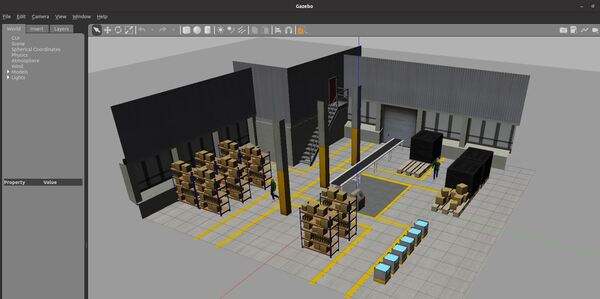
\includegraphics[width=0.8\textwidth]{warehouseEnvironment.jpg}
    \caption{The warehouse world environment [TODO better image]} \label{fig:warehouseWorld}
\end{figure}

The House world, shown in the figure \ref{fig:smallHouse}, represents a typical small, fully equipped apartment. Compared to the warehouse, this environment is significantly smaller and contains more various objects of different shapes and colors. Many of the typical household robots, like robotic vacuum cleaners, will deal with environments like this.\par

\begin{figure}[htpb]
    \centering
    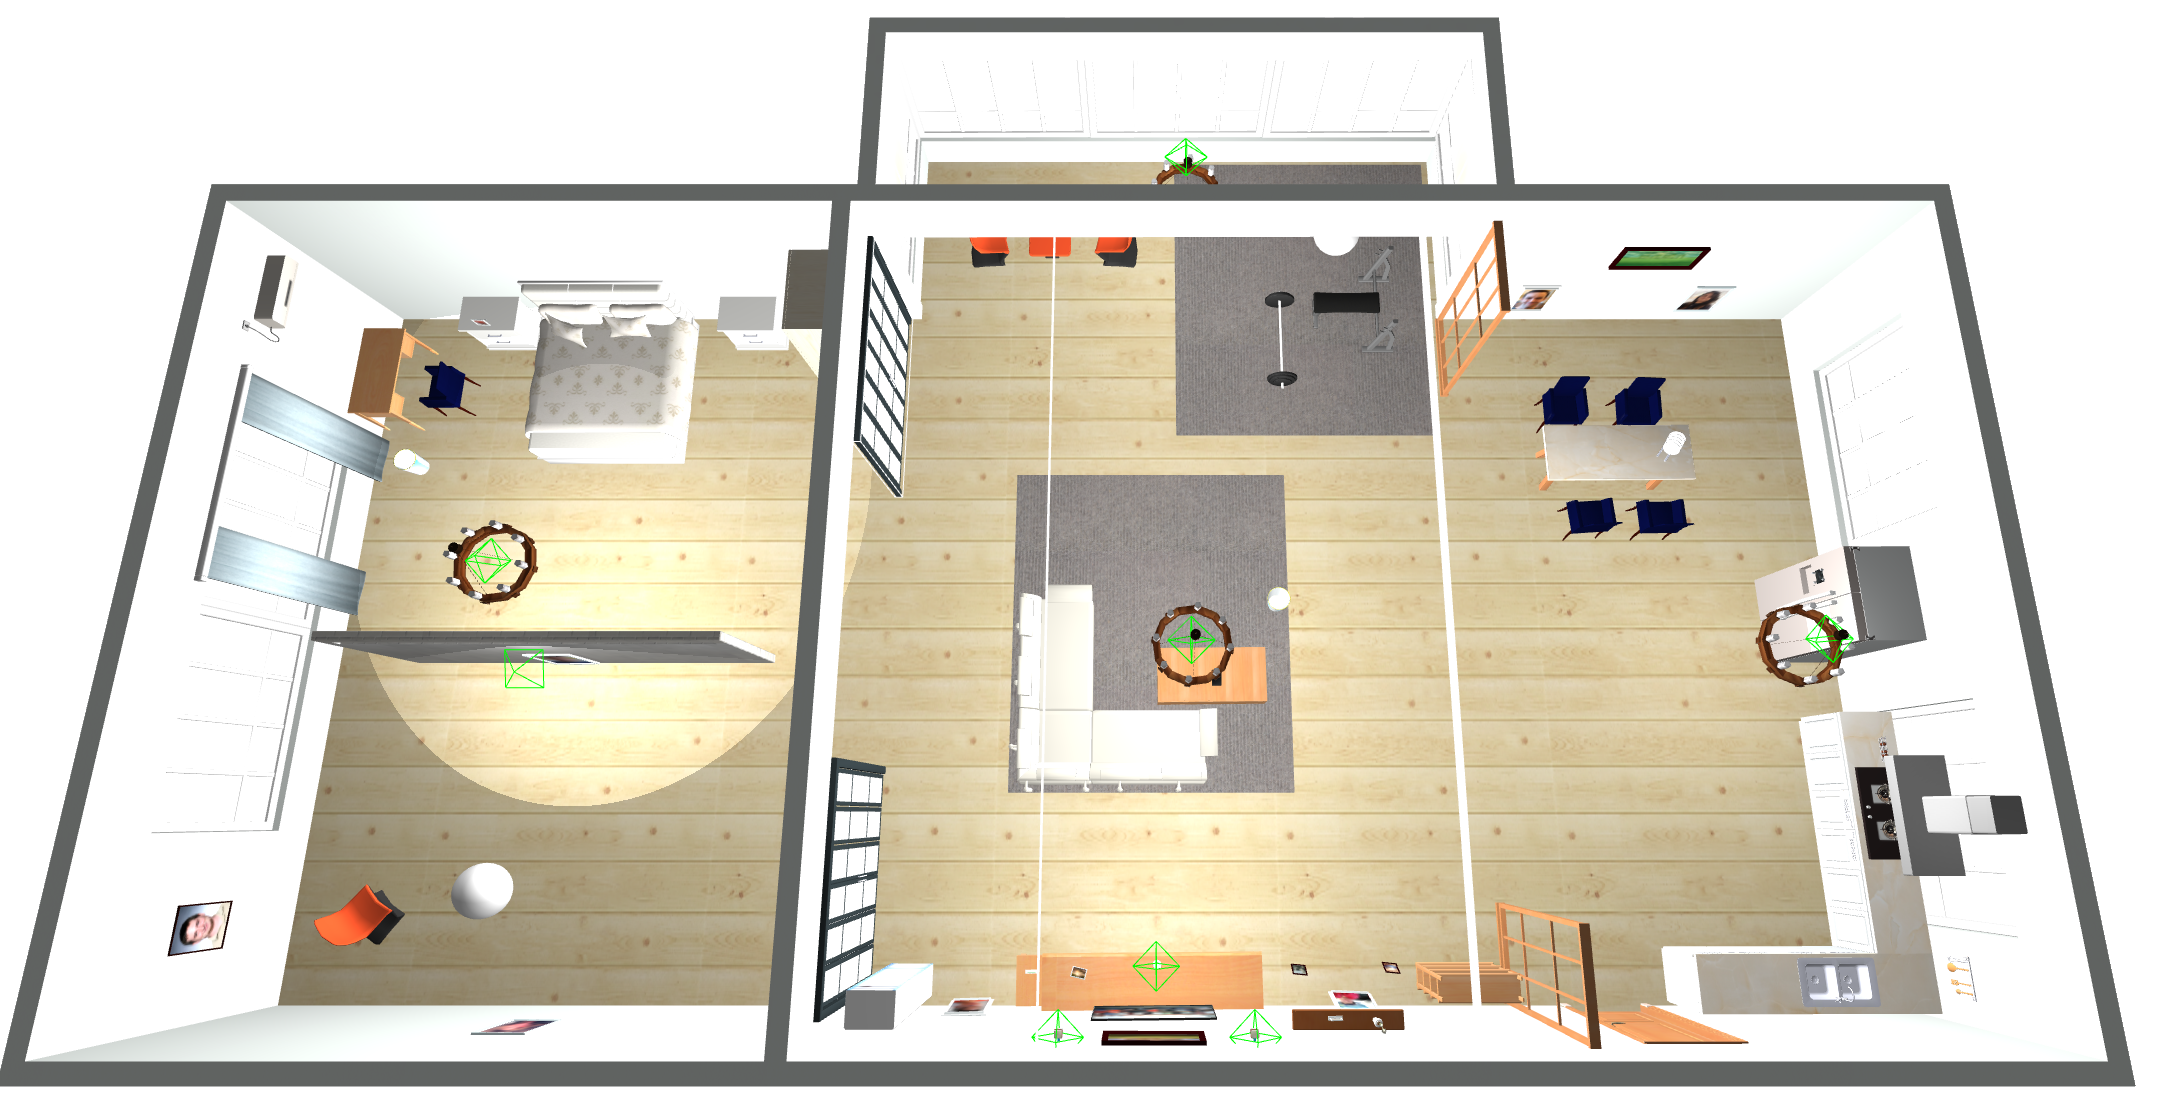
\includegraphics[width=0.8\textwidth]{smallHouse.png}
    \caption{The small house world environment [TODO ref]} \label{fig:smallHouse}
    % https://github.com/aws-robotics/aws-robomaker-small-house-world/blob/ros1/docs/images/gzweb_aws_house.png
\end{figure}

Finally, the hospital world, shown in the figure \ref{fig:hospitalWorld}, is a large, mostly empty environment from the hospital building. This environment is mostly symmetric and contains many places that look very similar, even if they are at opposite building sites. This environment was included mainly to test the algorithm's robustness against these symmetric places. Furthermore, this environment is a typical representation of any office or similar public building.\par

\begin{figure}[htpb]
    \centering
    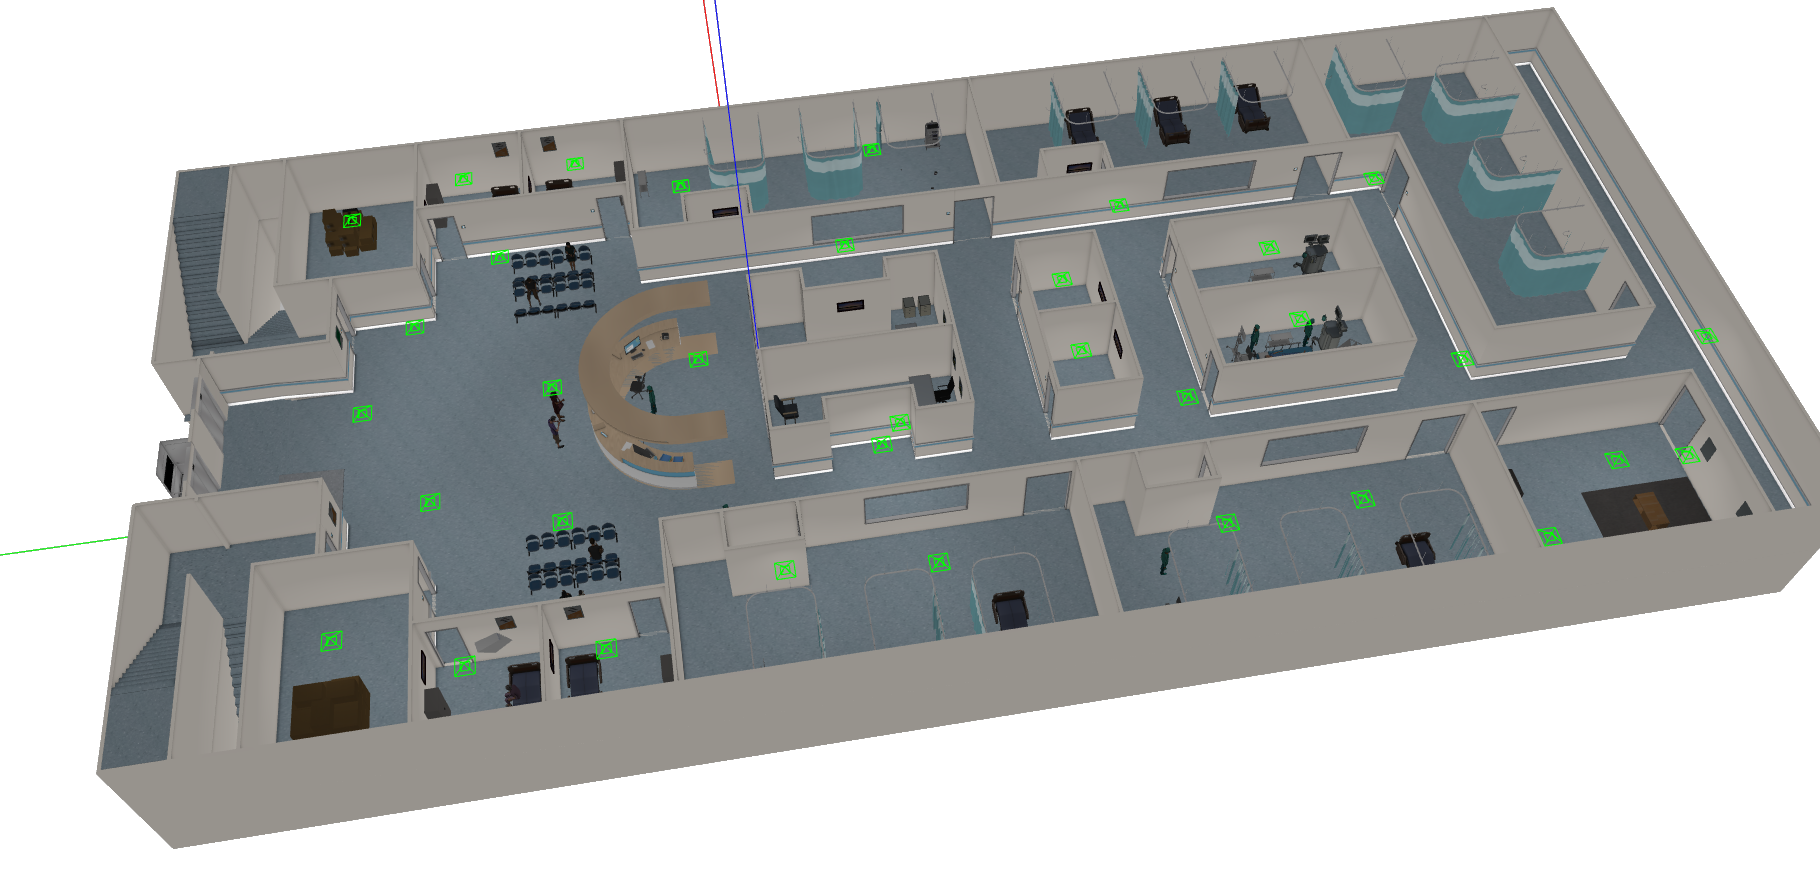
\includegraphics[width=0.8\textwidth]{Hospital.png}
    \caption{The hospital world environment [TODO ref]} \label{fig:hospitalWorld}
    % https://chowdera.com/2022/04/202204111258552961.html
\end{figure}

The algorithms were tested in each of the presented environments with several minutes long robot runs. The robot's trajectory was chosen so that the robot visits the same places several times to test the place recognition algorithm properly. All the robot runs were saved in rosbag files to ensure the repeatability of each experiment. Furthermore, every experiment for every metric presented further in this chapter has been performed on the same trajectory.\par
The dataset generated for the parameter tuning, described in the section \ref{section:parameterTuning}, and for the training of the neural networks, described in the section \ref{section:nnTraining}, were generated exclusively from the warehouse environment. The datasets' trajectory was entirely different from the trajectory used for the performance testing, but the type of the objects remained similar. In these datasets were no scenes from the other two environments.